\documentclass{article}
\usepackage[utf8]{inputenc}
\usepackage{graphicx}

\title{EasyTikZ\\
\normalsize{converting "{}Kritzeleien"{} to TikZ-code}}
\author{
    \begin{tabular}{l r}
        Robin Holländer& Niklas Heyne  \\
        108014394238 & 108013208773 
    \end{tabular}
}
\date{\today}

\begin{document}
\maketitle
\pagebreak
\section{requirements}
\subsection*{raster graphics $\rightarrow$ semantic model}
\subsubsection*{necessary} 
\begin{enumerate}
    \item detect and recognize a limited number of shapes
    \item detect connections between shapes
    \item detect and recognize labels inside of shapes
    \item detect freely positioned text
    \item basic automatic alignment of structures
\end{enumerate}
\subsubsection*{expected} 
\begin{enumerate}
    \item recognize arbitrary polygons < 6 vertices (within reasonable limits)
    \item robustness against discontinuous lines
    \item better automatic alignment of structures
    \item recognize specific parameters for shapes (rounded corners, fixed angle rotations, line thickness)
    \item recognize relative text position in shapes
\end{enumerate}
\subsubsection*{treats}
\begin{enumerate}
    \item allow for parameterized alignment thresholds
    \item recognize groups of identical shapes
    \item recognize different endpoints of connectors
\end{enumerate}
\subsection*{semantic model $\rightarrow$ TikZ code}
\subsubsection*{necessary}
\begin{enumerate}
    \item human readable
    \item intuitive structure of code
    \item generation of shapes
    \item generation of connections
    \item generation and targeted placement of text
\end{enumerate}
\subsubsection*{expected}
\begin{enumerate}
    \item easily adjustable cosmetic preferences \\line thickness, possible grid etc.
    \item code optimization
\end{enumerate}
\subsubsection*{treats}
\begin{enumerate}
    \item use loops to better parameterize groups of shapes
    \item extend adjustment capabilities to store variables for group parameters
\end{enumerate}
\section{flowchart}
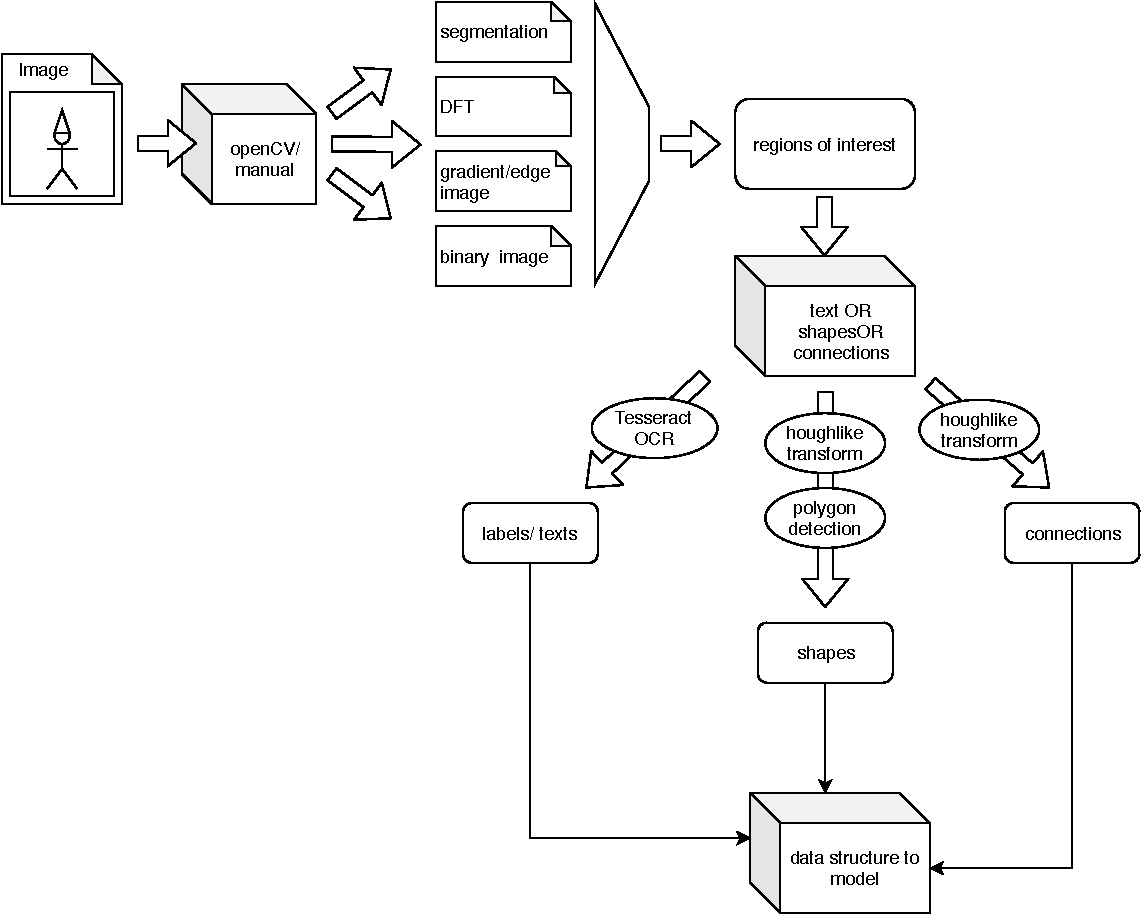
\includegraphics[width=\textwidth]{./img/FlowchartTikZ.pdf}
\section{Progress}
\subsection{18.04. - 24.04.}
\end{document}
